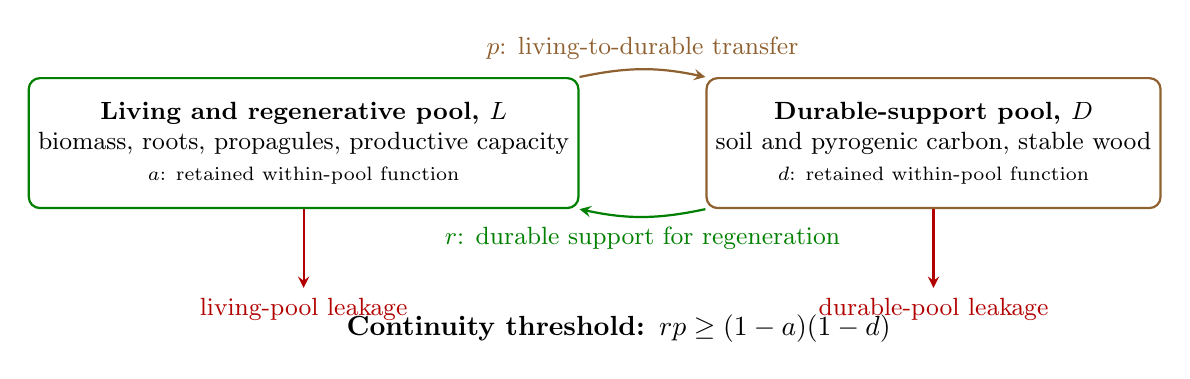
\begin{tikzpicture}[>=stealth,thick,font=\small]
\node[draw=green!50!black,rounded corners,minimum width=5.1cm,minimum height=1.65cm,align=center] (L) at (0,0) {\textbf{Living and regenerative pool, $L$}\\biomass, roots, propagules, productive capacity\\{\scriptsize $a$: retained within-pool function}};
\node[draw=brown!75!black,rounded corners,minimum width=5.1cm,minimum height=1.65cm,align=center] (D) at (8.0,0) {\textbf{Durable-support pool, $D$}\\soil and pyrogenic carbon, stable wood\\{\scriptsize $d$: retained within-pool function}};
\draw[->,brown!75!black] (L.north east) to[bend left=12] node[above] {$p$: living-to-durable transfer} (D.north west);
\draw[->,green!50!black] (D.south west) to[bend left=12] node[below] {$r$: durable support for regeneration} (L.south east);
\draw[->,red!70!black] (L.south) -- ++(0,-1.0) node[below] {living-pool leakage};
\draw[->,red!70!black] (D.south) -- ++(0,-1.0) node[below] {durable-pool leakage};
\node[font=\bfseries] at (4,-2.35) {Continuity threshold: $rp \geq (1-a)(1-d)$};
\end{tikzpicture}
